En aquest capítol farem una breu introducció a les llibreries i eines utilitzades per dur a terme el projecte. També veurem alguns dels motors de videojocs més utilitzats, i analitzarem les diferències respecte al nostre.
\section{Motors}
\subsection{Unity}
\begin{center}
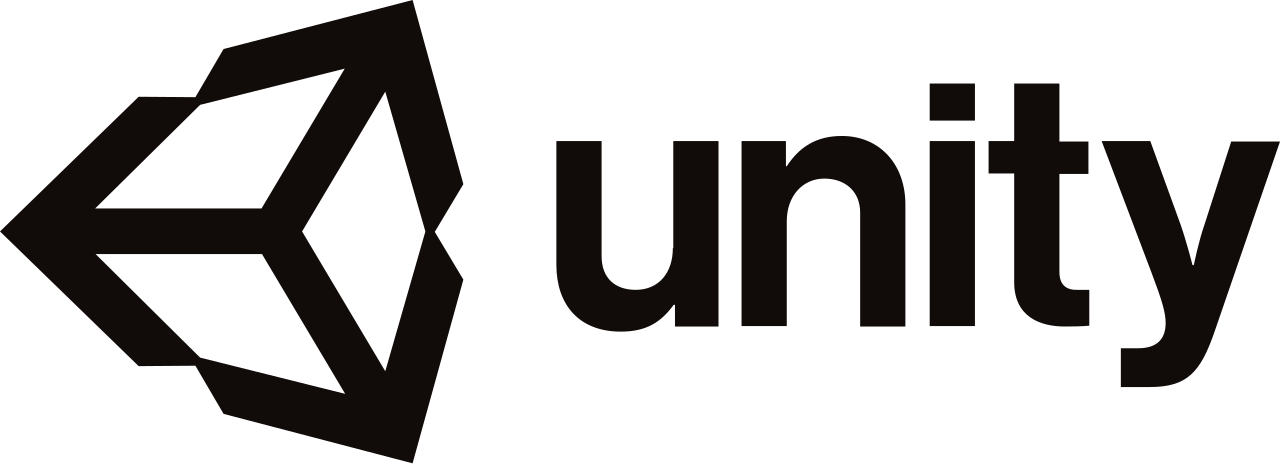
\includegraphics[scale=0.22]{unitylogo}
\end{center}
Unity és un motor de videojocs multiplataforma publicat per Unity Technologies l'any 2005. Des d'aleshores ha guanyat una gran popularitat, i ha passat a ser un dels gegants de la indústria.
Amb l'objectiu d'oferir un motor accessible a més desenvolupadors, Unity va ser un dels promotors de l'explosió de videojocs \textit{indie} al voltant del any 2007.
Unity és de codi propietari tot i tenir alguna part publicada amb llicència de només referència, i ofereix subscripcions de pagament així com una versió gratuïta per a petits desenvolupadors.
\\
El motor està construït al voltant d'un editor gràfic 3D, el qual exposa gran part de la funcionalitat de manera visual, evitant la necessitat de modificar codi directament.
Es pot programar tant en C++ i C#, com amb el llenguatge de scripting visual Bolt.
\\
Unity ofereix suport multiplataforma per a totes les plataformes de videojocs modernes. Estàn incloses Windows, Linux, Mac OS, Android, iOS, Nintendo Switch i Xbox One.
\\
La llista de jocs famosos creats en Unity està continuament en expansió, a continuació llistem alguns d'ells:
\begin{itemize}
  \item Kerbal Space Program
  \item Hearthstone
  \item Cuphead
  \item Cities Skylines
  \item Hollow Knight
  \item Enter the Gungeon
  \item Ori and the Blind Forest
\end{itemize}

\begin{figure}[h]
  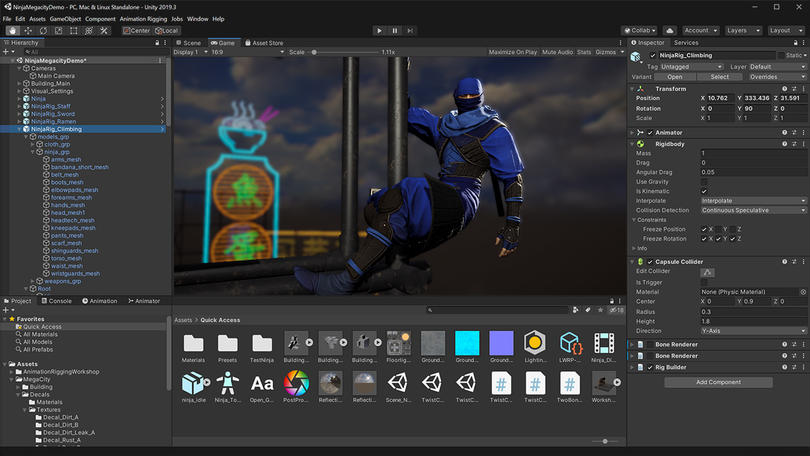
\includegraphics[scale=0.4]{unitycaptura}
  \caption{Captura de pantalla del editor Unity 2019.3}
\end{figure}

\subsection{Unreal Engine}
\begin{center}
  
\includegraphics[scale=0.1]{unreallogo}
\end{center}
Unreal Engine és un motor de videojocs desenvolupat per Epic Games. Desenvolupat inicialment per Tim Sweeney l'any 1995 com a motor pel joc Unreal, l'Unreal Engine ha passat a ser un dels motors més utilitzats per a jocs AAA.
El motor disposa d'una interfície gràfica des d'on es desenvolupen els jocs, i permet als desenvolupadors utilitzar codi C++, o fer servir el seu propi llenguatge de scripting visual anomenat Blueprint.
\\
Unreal Engine ofereix tant una modalitat gratuïta per a petits desenvolupadors, com modalitats de pagament amb les que donen accés al codi font.
La llista de jocs AAA que utilitzen Unreal Engine és immensa, però aquí llistem alguns dels més importants:
\begin{itemize}
  \item Rocket League
  \item Fortnite
  \item PUBG
  \item Saga Gears of War
  \item Saga Bioshock
  \item Saga Borderlands
\end{itemize}

Com Unity, Unreal Engine ofereix suport multiplataforma per a Windows, Mac, Linux, Android, iOS, Nintendo Switch, PS4 i Xbox One.
\begin{figure}[h]
  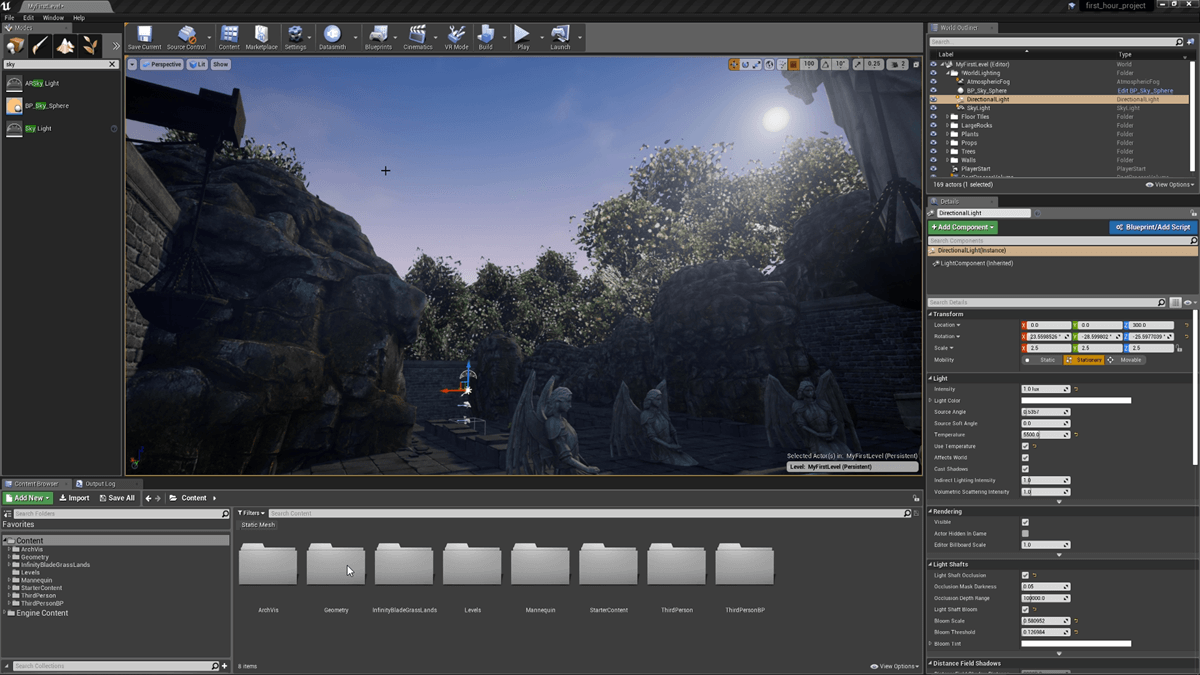
\includegraphics[scale=0.3]{unrealcaptura}
  \caption{Captura de pantalla del editor d'Unreal Engine 4}
\end{figure}
\subsection{Godot}
\begin{center}
  
\includegraphics[scale=0.2]{godotlogo}
\end{center}
Godot és motor de videojocs originalment creat per Juan Linietsky i Ariel Manzur. Tot i ser comparativament molt més petit que Unity i Unreal, recentment està rebent grans actualitzacions que el poden apropar al nivell dels altres 2.
A diferència d'Unity i Unreal, Godot és distribuït sota la llicència de codi lliure MIT, i és publicat en un repositori de Github.
Ofereix una interfície gràfica per editar projectes, i tot i estar inicialment orientat a videojocs 2D, suporta també projectes en 3D, amb la major concentració del desenvolupament recent centrant-se en aquesta part.
Pot ser programat a través d'un editor de scripts visual, C#, el seu propi llenguatge anomenat GDScript, o a través de GDNative, que és una interfície que permet interactuar amb llenguatges compilats tot i que només C++ està suportat de manera oficial.
Oficialment suporta compilacions per a Windows, Mac OS, Linux, Android, iOS i web a través de emscripten. Tot i que oficialment no suporta cap consola, hi ha tercers que ofereixen suport per a Nintendo Switch, PS4 i Xbox One sempre que es disposi del SDK oficial.
\subsection{Decisió}
Degut a que cap dels motors de videojocs principals actuals compleix els principals objectius del nostre projecte, creiem que el nostre motor pot ocupar un espai que actualment no està cobert en el sector.
\section{Llenguatges}
\subsection{C}
\subsection{C++}
\subsection{Rust}
\section{Llibreries}
\subsection{Multimèdia}
\subsubsection{SDL2}
\begin{center}
  
\includegraphics[scale=0.15]{sdl2logo}
\end{center}
Simple DirectMedia Layer 2 és una capa d'abstracció de hardware multiplataforma. Ofereix al programador una API per gestionar audio, video, dispositius d'entrada i finestres entre d'altres. La seva funció és facilitar el desenvolupament de projectes multiplataforma, separant el codi específic de cada dispositiu a dins de la llibreria, i oferint crides homogènies a través d'una API.
Tot i que la API és per a C, és perfectament utilitzable des de C++. Es distruibueix amb llicència Zlib, i suporta Linux, Windows, Mac OS, emscripten, iOS i Anrdoid entre d'altres. De forma no oficial també hi ha suport per a Nintendo Switch, desenvolupat per membres de la comunitat.
\subsubsection{SFML}
\begin{center}
  
\includegraphics[scale=0.5]{sfmllogo}
\end{center}
Simple and Fast Multimedia Library és una altre capa d'abstracció de hardware multiplataforma similar a SDL. Es diferencia respecte SDL en ser lleguerament més orientada a C++. També és publicada sota llicència Zlib, però actualment no existeix suport per a Nintendo Switch.
\subsubsection{Decisió}
Degut a la falta de suport per a Nintendo Swich de SFML, hem decidit triar SDL2 com a capa multimèdia pel projecte. Com que nosaltres també afegirem una capa d'abstracció de hardware pròpia al projecte, podríem haver escollit SFML per la versió de PC i SDL2 per a Nintendo Switch, però hagués suposat un esforç extra que no hauria aportat cap benefici al projecte.

\subsection{FastNoise}
FastNoise és una llibreria de generació de gradients de soroll per C++. Permet de forma senzilla generar sorolls Value, Perlin, Simplex, Celular i Blanc tant en formats 2D com 3D. També permet soroll Simplex en 4D, i habilita la combinació de diferents nivells de soroll amb moviment fraccional Brownià.
\subsection{EnTT}
\begin{center}
  
\includegraphics[scale=0.4]{enttlogo}
\end{center}
EnTT és un framework de gestió de Entity Component System per C++. Està publicat sota la llicència MIT, i està en actiu desenvolupament a Github. A part del ECS també inclou diverses altres eines, però nosaltres farem ús exclusiu del ECS. Entre d'altres, és utilitzat per la versió Bedrock de Minecraft.
\subsection{ReactPhysics3D}
ReactPhysics3D és un motor de física per a simulacions i jocs en C++. Està en actiu desenvolupament a Github, i és publicat sota la llicència MIT. Tot i que RP3D ofereix la possibilitat de fer tots els càlculs de física de forma autònoma, nosaltres només l'utilitzarem per a detecció de co\lgem isions i farem la resta de càlculs nosaltres degut a la naturalesa del nostre motor.
\subsection{nlohmann/json}
JSON for Modern C++, conegut popularment per la seva adreça de Github com a nlohmann/json és una lleugera llibreria que facilita la manipulació d'arxius JSON des de C++. Està en actiu desenvolupament i es troba publicat sota la llicència MIT.
\subsection{IceCream-Cpp}
IceCream-Cpp és una molt petita llibreria que assisteix a l'hora de fer debugging a través de la consola. Alguns errors, per la seva naturalesa, són més fàcils de diagnosticar i arreglar a través de text a la consola en una configuració Release, que no pas amb un debugger. Aquesta llibreria va ser afegida a la meitat del projecte al trobar-la per casualitat, i descobrir que podia ser útil.
\subsection{DevkitA64}
\begin{center}
  
\includegraphics[scale=0.5]{devkitprologo}
\end{center}
DevkitA64 és un \textit{toolchain} publicat per l'equip de DevkitPro que permet, junt a libnx, compilar projectes C++ per a la Nintendo Switch. Es troba sota la llicència ISC, que és funcionalment equivalent a BSD 2C i MIT.
\subsection{Qt Creator}

\subsection{Visual Studio}

